\section{Technical Experimentation}
In this section, we will present the field we previously described with illustrations. 
\begin{figure}[h!]
    \centering
    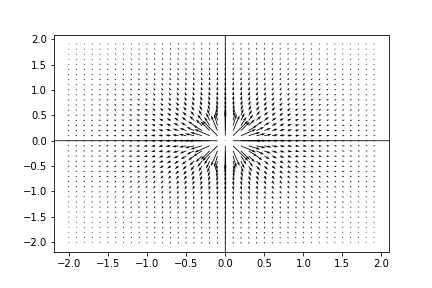
\includegraphics[width=0.48\textwidth]{Images/simplesource.png}
    \caption{Simple Type 1 irrotational source}
    \label{fig:simplesource}
\end{figure}
The field in figure \ref{fig:simplesource} was drawn by computing the gradient of $V_1$ with $(\tilde{{x}_{1}}, \tilde{{x}_{2}}) = (0,0)$.

\begin{figure}[h!]
    \centering
    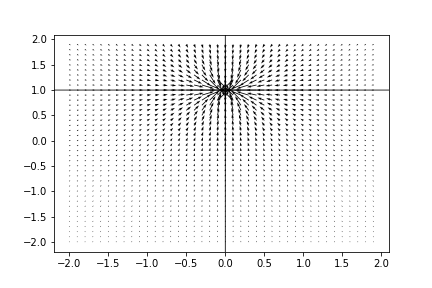
\includegraphics[width=0.48\textwidth]{Images/simplesink01.png}
    \caption{Simple Type 1 irrotational sink}
    \label{fig:simplesink}
\end{figure}
The field in figure \ref{fig:simplesink} is a sink field at $(0,1)$, it is similar to the source field in figure \ref{fig:simplesource} but with opposite sign.

\begin{figure}[h!]
    \centering
    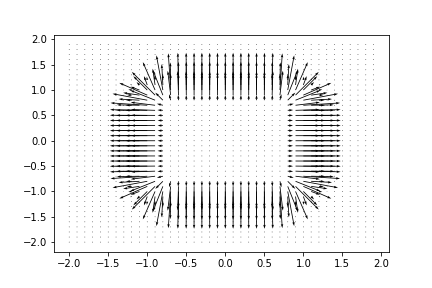
\includegraphics[width=0.48\textwidth]{Images/irrotafromshaping.png}
    \caption{irrotational field from shaping}
    \label{fig:irrotafromshaping}
\end{figure}
The field in figure \ref{fig:irrotafromshaping} has been generated by computing the gradient of the shaping function of a superquadratic: 
\begin{align}
    H=(x_1-\tilde{{x}_{1}})^n+(x_2-\tilde{{x}_{2}})^n \\
    F=\frac{1}{1+(\frac{1}{L}H^{\frac{1}{n}})^m}
\end{align}
As stated in \cite{mcinnes2003velocity}, when $m\gg1$, the edge of the shaping function gets thinner. Higher values of $n$ result in more rectangular shapes whereas $n=2$ describes the shaping function of a sphere.

Both these fields are type 1 irrotational solutions of the Laplace equation.

By adding the irrotational sink from figure \ref{fig:simplesink} and the irrotational field from shaping function in figure \ref{fig:irrotafromshaping} we obtain a good representation in figure \ref{fig:irrotafromshapingwithsink} of what the velocity field will look like when close to the target point. 
\begin{figure}[h!]
    \centering
    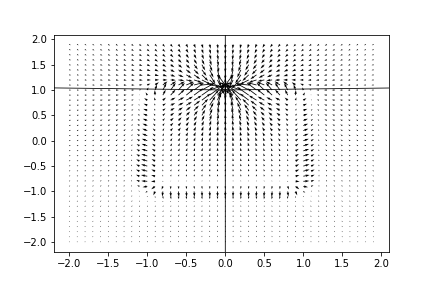
\includegraphics[width=0.48\textwidth]{Images/irrotashapingwithsink.png}
    \caption{irrotational field from shaping with sink}
    \label{fig:irrotafromshapingwithsink}
\end{figure}

The shaping function is mainly used to generate a vortex field around an obstacle, as explained in the paper. It is given by: 
\begin{equation}
    v_2=-\frac{\partial{F}}{\partial{x_2}}e_1 + \frac{\partial{F}}{\partial{x_1}}e_2
\end{equation}
Here, $e_1$ and $e_2$ are an orthonormal basis. \\ 
We can see in figure \ref{fig:rotafromshaping} an example of vortex field around a super quadriatic.
\begin{figure}[h!]
    \centering
    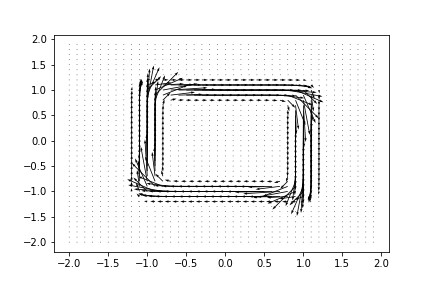
\includegraphics[width=0.48\textwidth]{Images/rotafromshaping.png}
    \caption{Solenoidale field from shaping function}
    \label{fig:rotafromshaping}
\end{figure}

As explained in section 2, after we made contact, we stop using the potential based field and we use the spherical field to maintain 
contact with the desired force.
Figure \ref{fig:spherical} represents an example of such a field where the red point is the optimal position to apply the pressure, the blue arrows are the velocity field vectors and the center of the sphere is the point where the pressure is applied

\begin{figure*}[h!]
    \centering
    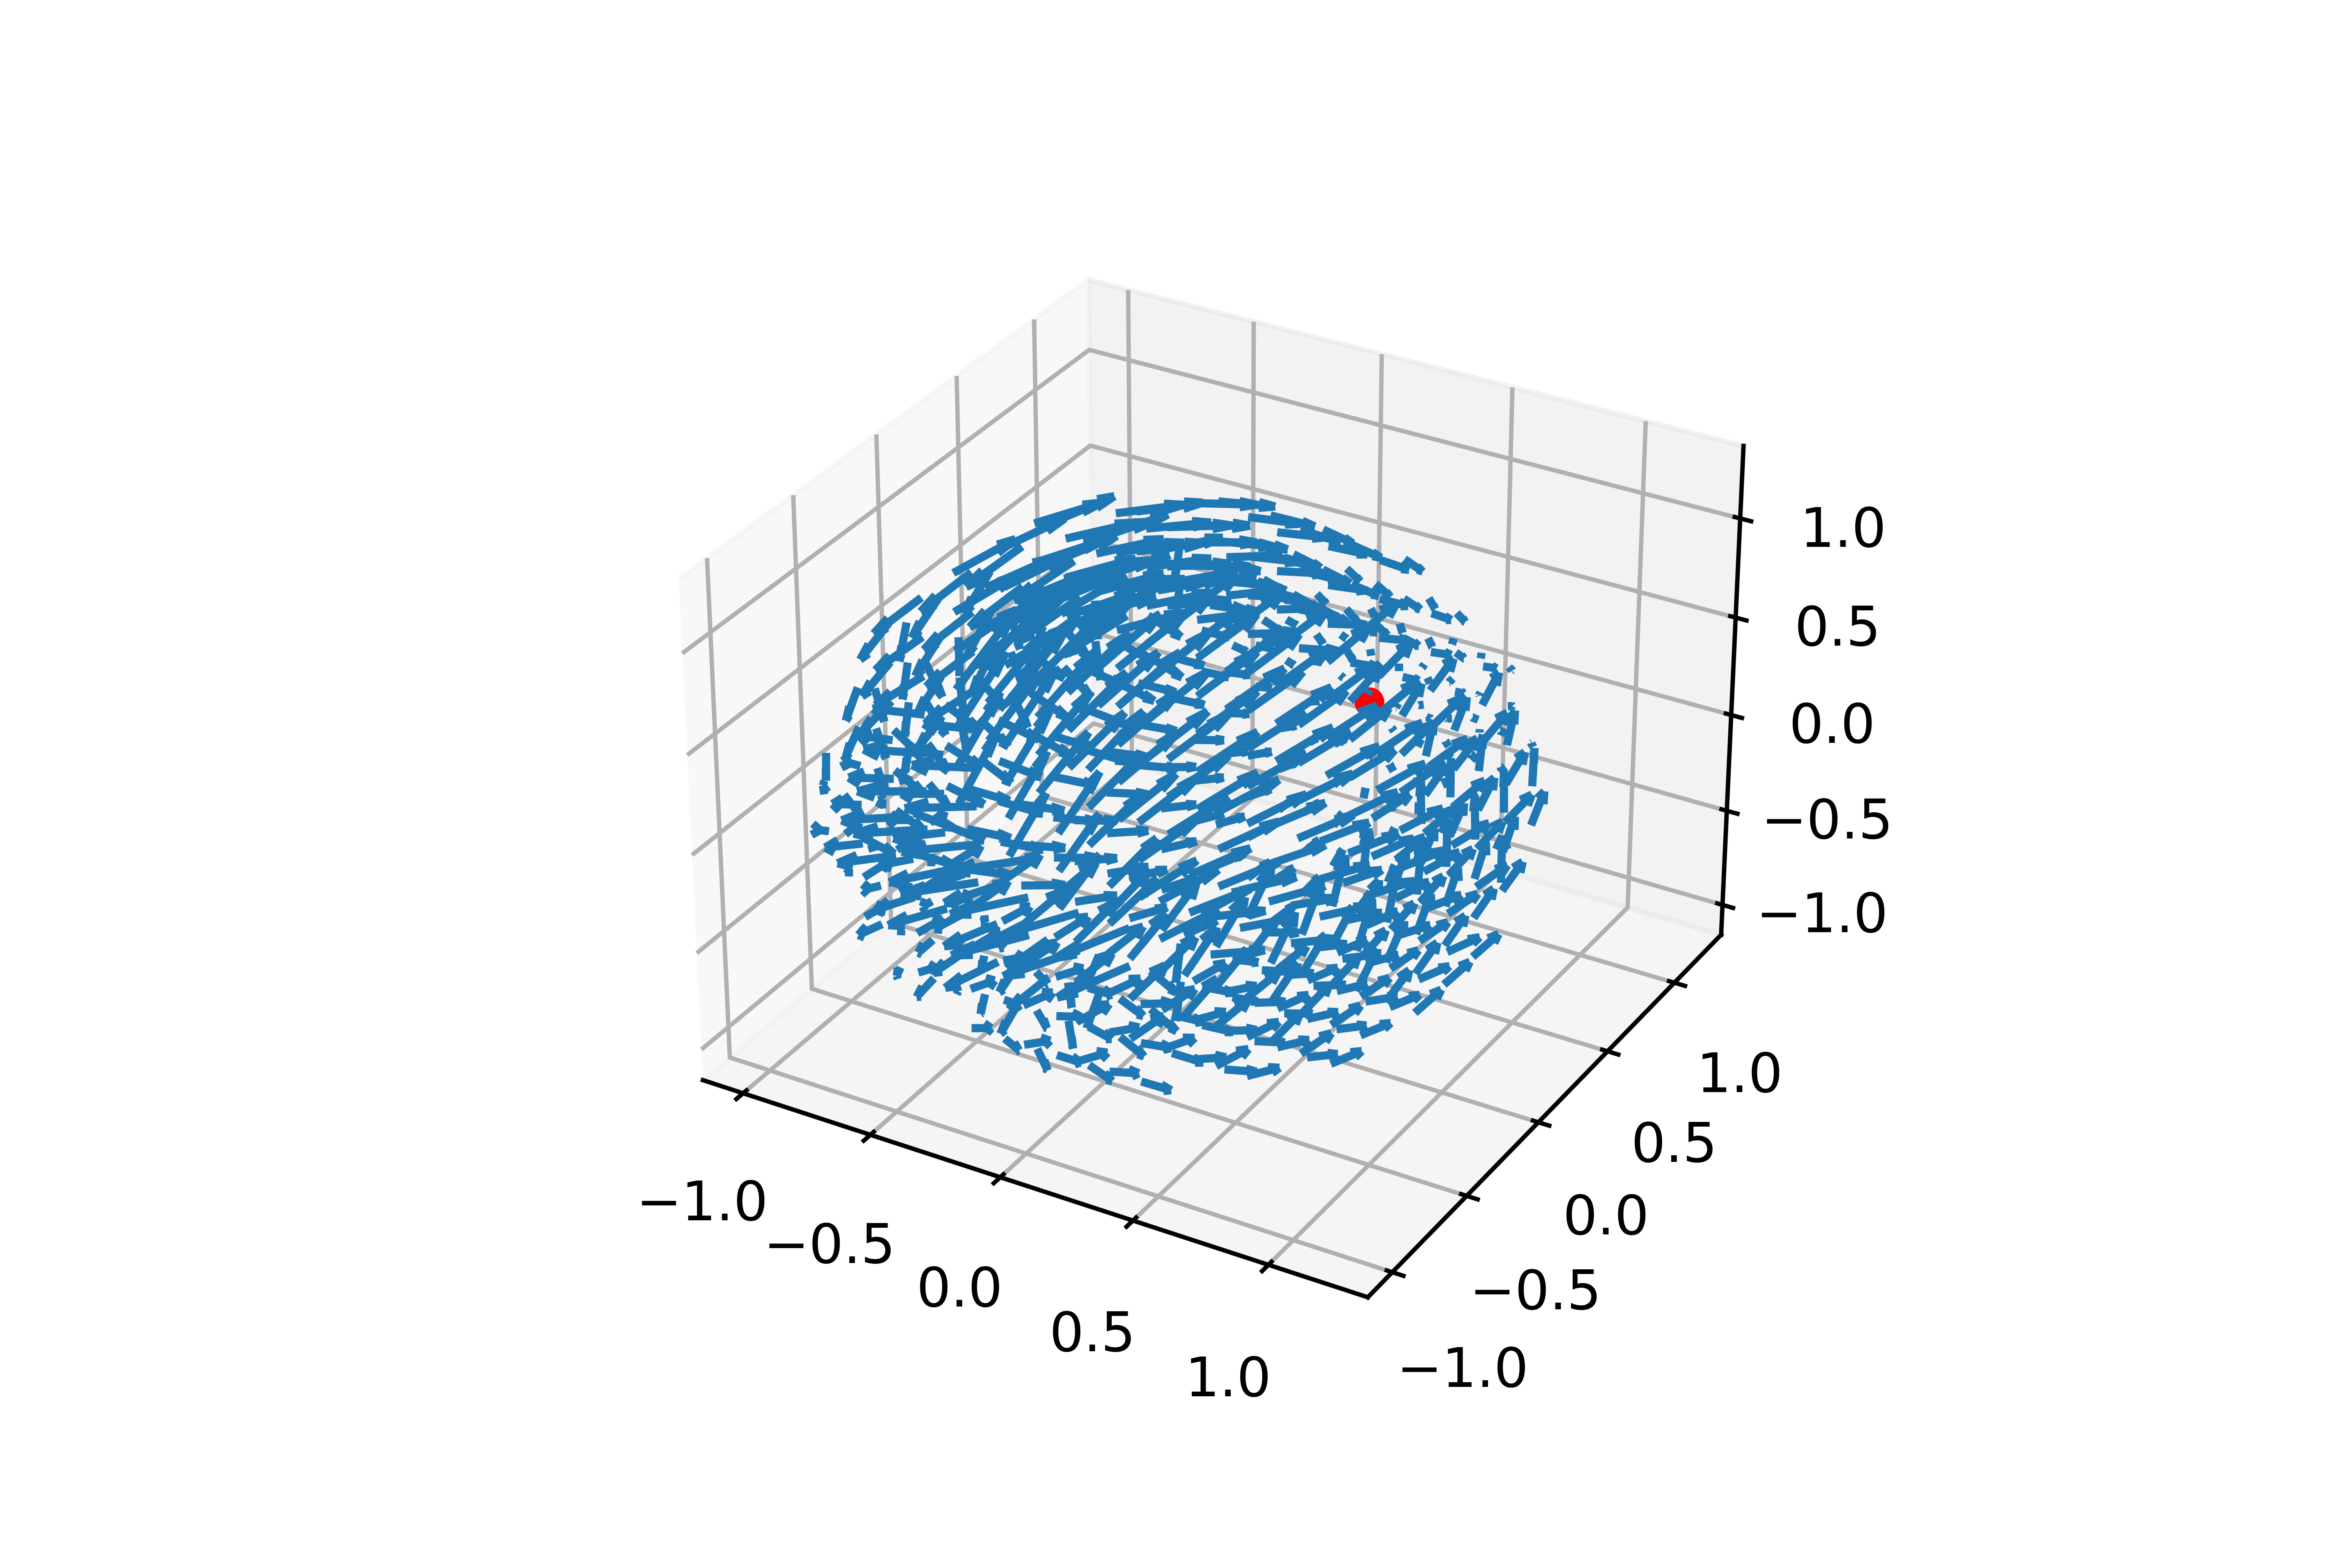
\includegraphics[scale=1.3]{Images/sphericalfield.png}
    \caption{Spherical contact field}
    \label{fig:spherical}
\end{figure*}
